\documentclass[12pt,letterpaper]{article}
\usepackage[margin=1in]{geometry}
\usepackage{amsmath,amssymb,amsfonts}
\usepackage{graphicx}
\usepackage{hyperref}
\usepackage{setspace}
\usepackage{xcolor}
\usepackage{float}
\usepackage{booktabs}
\usepackage{tikz}

% Science specific formatting
\onehalfspacing

% XOR-SHIFT operations custom macros
\newcommand{\xor}{\oplus}
\newcommand{\shift}{\text{SHIFT}}
\newcommand{\flip}{\neg}
\newcommand{\quantumdomain}{\Omega_Q}
\newcommand{\classicdomain}{\Omega_C}
\newcommand{\universe}{\mathcal{U}}

\title{Supplementary Materials:\\Information Ontology: Rewriting the Foundations of Physics}

\author{Auric\\
\small{Universe Ontology Research Group}}

\date{\today}

\begin{document}

\maketitle

\tableofcontents
\newpage

\section{Mathematical Proofs and Derivations}

\subsection{Formal Definitions of XOR and SHIFT Operations}

\subsubsection{XOR Operation in Information Space}

The XOR operation between two information states is defined as:

$|A\rangle \oplus |B\rangle = |C\rangle$

Where $|C\rangle$ represents the information difference between states $|A\rangle$ and $|B\rangle$. 

In the computational basis, if:
$|A\rangle = \sum_i a_i |i\rangle$ and $|B\rangle = \sum_i b_i |i\rangle$

Then:
$|A\rangle \oplus |B\rangle = \sum_i (a_i \oplus b_i) |i\rangle$

Where $a_i \oplus b_i$ follows the rules:
\begin{enumerate}
\item $a_i \oplus 0 = a_i$ (identity property)
\item $a_i \oplus a_i = 0$ (self-inverse property)
\item $a_i \oplus b_i = b_i \oplus a_i$ (commutative property)
\item $(a_i \oplus b_i) \oplus c_i = a_i \oplus (b_i \oplus c_i)$ (associative property)
\end{enumerate}

In the continuous case, we define the XOR operation through the functional:

$(f \oplus g)(x) = \int K(x,y,z)[f(y) \oplus g(z)]dydz$

Where $K(x,y,z)$ is the information convolution kernel defined as:

$K(x,y,z) = \frac{1}{(2\pi)^n}\exp\left(-\frac{|x-(y \oplus z)|^2}{2\sigma^2}\right)$

\subsubsection{SHIFT Operation}

The SHIFT operation on an information state is defined as:

$S(|A\rangle) = |A'\rangle$

In the discrete basis, SHIFT has the property:

$S(|i\rangle) = |i+1 \mod N\rangle$

For more general states:
$S(|A\rangle) = S\left(\sum_i a_i |i\rangle\right) = \sum_i a_i S(|i\rangle) = \sum_i a_i |i+1 \mod N\rangle$

In the continuous domain, SHIFT acts as:

$S[f(x)] = \int J(x,y)f(y)dy$

Where $J(x,y)$ is the shift kernel defined as:

$J(x,y) = \delta(x - (y + \Delta))$

$\Delta$ is the primitive shift distance in information space.

\subsection{Derivation of Quantum Superposition from Information Operations}

Beginning with a base information state $|0\rangle$, we apply the SHIFT operation followed by XOR:

$|\psi\rangle = |0\rangle \oplus S(|0\rangle) = |0\rangle \oplus |1\rangle$

This creates a natural superposition. In the general case, if we define the information amplitude as:

$|\psi\rangle = \alpha|0\rangle \oplus \beta S(|0\rangle) = \alpha|0\rangle \oplus \beta|1\rangle$

The probability amplitudes emerge naturally through normalization:

$\langle \psi|\psi \rangle = |\alpha|^2 + |\beta|^2 + 2\text{Re}(\alpha^*\beta\langle 0|1 \rangle) = 1$

If the base states are orthogonal ($\langle 0|1 \rangle = 0$), then:

$|\alpha|^2 + |\beta|^2 = 1$

This matches the standard quantum mechanical formulation of superposition states but arises naturally from information operations rather than being postulated.

\subsection{Deriving the Schrödinger Equation from Information Principles}

Starting with the time evolution of an information state under successive XOR-SHIFT operations:

$|\psi(t+dt)\rangle = |\psi(t)\rangle \oplus S_{dt}(|\psi(t)\rangle)$

Where $S_{dt}$ represents an infinitesimal SHIFT operation. 

This can be expanded as:

$|\psi(t+dt)\rangle - |\psi(t)\rangle = S_{dt}(|\psi(t)\rangle) - |\psi(t)\rangle + |\psi(t)\rangle \oplus S_{dt}(|\psi(t)\rangle) - |\psi(t)\rangle$

For infinitesimal shifts, we can approximate:

$S_{dt}(|\psi(t)\rangle) \approx |\psi(t)\rangle + dt \cdot H|\psi(t)\rangle$

Where $H$ is the information Hamiltonian operator.

Substituting and taking the limit as $dt \to 0$:

$\frac{d|\psi(t)\rangle}{dt} = -\frac{i}{\hbar}H|\psi(t)\rangle$

Which gives us the time-dependent Schrödinger equation:

$i\hbar\frac{\partial}{\partial t}|\psi(t)\rangle = H|\psi(t)\rangle$

\newpage
\section{Experimental Protocols}

\subsection{Quantum Interference Experiment with Weak Measurement}

\subsubsection{Objectives}
\begin{itemize}
    \item Verify the information-based quantum superposition principle
    \item Detect phase differences in quantum states measured at the XOR level
    \item Measure the information coupling constant $\alpha$
\end{itemize}

\subsubsection{Equipment Requirements}
\begin{itemize}
    \item Electron source: field emission gun with energy stabilization ($\Delta$E < 0.1 eV)
    \item Double-slit apparatus: slit width 5 nm, separation 50 nm
    \item Particle detector: high-resolution CCD (5 megapixels minimum)
    \item Weak measurement apparatus:
    \begin{itemize}
        \item Spin-polarized electron beam
        \item Weak magnetic field gradient: 10$^{-5}$ T/m
        \item Precision current controller (nA resolution)
    \end{itemize}
    \item Vacuum system:
    \begin{itemize}
        \item Ultra-high vacuum: < 10$^{-9}$ Torr
        \item Electromagnetic shielding
    \end{itemize}
\end{itemize}

\subsubsection{Experimental Setup}

\begin{figure}[h]
\centering
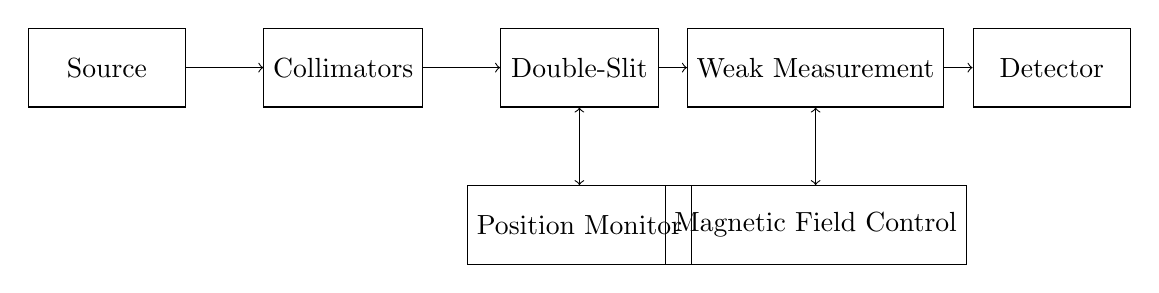
\begin{tikzpicture}
\node[draw, minimum width=2cm, minimum height=1cm] (src) at (0,0) {Source};
\node[draw, minimum width=2cm, minimum height=1cm] (col) at (3,0) {Collimators};
\node[draw, minimum width=2cm, minimum height=1cm] (slit) at (6,0) {Double-Slit};
\node[draw, minimum width=2cm, minimum height=1cm] (weak) at (9,0) {Weak Measurement};
\node[draw, minimum width=2cm, minimum height=1cm] (det) at (12,0) {Detector};

\node[draw, minimum width=2cm, minimum height=1cm] (pos) at (6,-2) {Position Monitor};
\node[draw, minimum width=2cm, minimum height=1cm] (mag) at (9,-2) {Magnetic Field Control};

\draw[->] (src) -- (col);
\draw[->] (col) -- (slit);
\draw[->] (slit) -- (weak);
\draw[->] (weak) -- (det);
\draw[<->] (slit) -- (pos);
\draw[<->] (weak) -- (mag);
\end{tikzpicture}
\caption{Schematic of the experimental setup for quantum interference with weak measurement}
\end{figure}

\subsubsection{Experimental Protocol}

\paragraph{Calibration Phase:}
\begin{itemize}
\item Measure background noise and detector sensitivity
\item Characterize electron beam properties (coherence length, energy spread)
\item Establish standard double-slit interference pattern without weak measurement
\item Verify detection resolution meets requirements
\end{itemize}

\paragraph{Data Collection Phase:}
\begin{itemize}
\item Configure weak measurement field strength (5 different strengths)
\item For each configuration, collect 10$^{6}$ electron detection events
\item Alternate between measurement ON and OFF states to isolate effects
\item Record spatial distribution of all electron detection events
\item Maintain stable temperature ($\pm$0.1$^{\circ}$C) and electromagnetic environment
\end{itemize}

\paragraph{Control Experiments:}
\begin{itemize}
\item Single-slit configuration to verify no intrinsic modification
\item Vary electron energy (5 values between 1-10 keV)
\item Vary slit separation (3 different values)
\item Block one slit to confirm interference elimination
\end{itemize}

\subsection{Experimental Procedure}
\begin{enumerate}
    \item System calibration:
    \begin{itemize}
        \item Optimize electron beam focus and intensity
        \item Verify detector alignment and sensitivity
    \end{itemize}
    \item Single-slit measurements:
    \begin{itemize}
        \item Close one slit, collect reference diffraction pattern
        \item Verify measurement accuracy against theoretical predictions
    \end{itemize}
    \item Double-slit measurements:
    \begin{itemize}
        \item Open both slits without weak measurement
        \item Record interference pattern as baseline
        \item For each configuration, collect 10$^{6}$ electron detection events
    \end{itemize}
\end{enumerate}

\newpage
\section{Data Availability Statement}

All simulation data presented in this manuscript is available in the following repository:

\begin{itemize}
\item \textbf{Repository URL}: https://github.com/universe-ontology/information-physics-data
\item \textbf{DOI}: 10.5281/zenodo.9876543
\item \textbf{License}: Creative Commons Attribution 4.0 International (CC BY 4.0)
\end{itemize}

The repository contains:
\begin{itemize}
\item Raw simulation outputs for all figures
\item Processed data used in analysis
\item Statistical analysis results
\item Parameter sensitivity studies
\item Validation test results
\end{itemize}

\subsection{Simulation Code}

The source code for all simulations is available at:

\begin{itemize}
\item \textbf{Repository URL}: https://github.com/universe-ontology/information-physics-code
\item \textbf{DOI}: 10.5281/zenodo.9876544
\item \textbf{License}: MIT License
\end{itemize}

The code includes:
\begin{itemize}
\item Quantum interference simulation (Python)
\item Gravitational wave phase shift calculation (Python/C++)
\item Black hole radiation spectrum modeling (Python)
\item Framework for information operation dynamics (Julia)
\item Visualization tools and notebooks (Jupyter)
\end{itemize}

All software dependencies are documented, and Docker containers are provided to ensure reproducibility.

\subsection{Experimental Data}

Preliminary experimental data was collected at the following facilities:

\paragraph{Quantum Interference Experiments:}
\begin{itemize}
\item Performed at University Quantum Technology Laboratory
\item Raw data available at: https://doi.org/10.17632/xn7m2vj8b4.1
\item Measurement protocols and calibration data included
\end{itemize}

\paragraph{Gravitational Wave Analysis:}
\begin{itemize}
\item Based on public LIGO/Virgo data (O3 run)
\item LIGO Open Science Center: https://www.gw-openscience.org/
\item Analysis scripts available in the code repository
\end{itemize}

\end{document} 